\subsection{Panda, demo variant «Pumpkin», November 2024}

Midterm will contain 6 problems. 
All the problems have equal weights. 
Midterm duration is 120 minutes. 
Closed book, one A4 cheatsheet is allowed.
All topics before (and including) bootstrap may be included. 

\begin{enumerate}
    \item You have estimated the linear regression 
    \[
    \hat y_i  = 3 + 0.2 x_i + 0.5 b_i - 0.7 c_i
    \]
    using big number of observations $n$. 
    Assume all Gauss~— Markov assumptions are satisfied. 

    The estimate of the covariance matrix of coefficients is 
    \[
    \begin{pmatrix}
        2.5 & -0.2 & 0.1  & 0 \\
        ?   &  4.5 & -0.1 & 0.1 \\
        ?   &   ?  & 3.2  & -0.1 \\
        ?   &   ?  &  ?   &  3.5 \\       
    \end{pmatrix}
    \]
    \begin{enumerate}
        \item Construct 95\% confidence interval for $\beta_x$.
        \item Construct 95\% confidence interval for conditional expected value of dependent variable if $x = 1$, $b = -1$, $c = 2$.
        \item Test that $\beta_x + \beta_b = 1$ against $\beta_ x + \beta_b \neq 1$ at 5\% significance level.
    \end{enumerate}


    \item Consider the simple regression model $y_i = \beta_0 + \beta_1 x_i + u_i$.
    Assume that Gauss~— Markov assumptions are satisfied.
    Let $z_i = \sqrt{x}_i$.

    Consider two estimators of $\beta_1$:
    \[
    \hb_1' = \frac{\sum_{i=1}^n(z_i - \bar z)y_i}{\sum_{i=1}^n(z_i - \bar z)x_i}, \quad \hb_1'' = \frac{\sum_{i=1}^n(z_i - \bar z)y_i}{\sum_{i=1}^n(z_i - \bar z)z_i}.
    \]
    \begin{enumerate}
        \item Calculate $\E(\hb_1' \mid x)$ and $\E(\hb_1'' \mid x)$. Are estimators unbiased conditionally on $x$?
        \item Are estimators $\hb_1'$ and $\hb_1''$ consistent?
    \end{enumerate}


    \item You have $300$ observations in total and you estimated the regression 
    \[
    \hat y_i = \hb_0 + \hb_1 x_i + \hb_2 v_i + \hb_3 w_i
    \]
    using different parts of your dataset.

    \begin{tabular}{rr}
        \toprule
        Observations & Result \\
        \midrule
        $1, \dots, 300$ & $\SSR = 300$, $\SST = 500$ \\
        $1, \dots, 200$ & $\SSR = 150$ \\
        $201, \dots, 300$ & $\SSR = 100$ \\
        \bottomrule
    \end{tabular}


    Assume for each case that Gauss~— Markov assumptions for the unrestricted model are satisfied. 
    Use 5\% critical level. 
    % Alternative hypothesis in each case is the violation of at least on constraint in $H_0$.

    \begin{enumerate}
        \item Test that $\beta_1 = \beta_2 = \beta_3 = 0$ for the whole dataset against alternative that at least one of the coefficients is non-zero.
        \item Test for the absence of a structural break between part one (observations $1$, \dots, $200$) and part two (observations $201$, \dots, $300$) of your dataset.
        Here in $H_0$ you assume that the relation $y_i = \beta_0 + \beta_1 x_i + \beta_2 v_i + \beta_3 w_i + u_i$
        holds for the whole dataset. 
        And in $H_1$ you assume that different linear models may be valid for the two parts of your dataset.
        \item Consider again $H_0$ that the relation $y_i = \beta_0 + \beta_1 x_i + \beta_2 v_i + \beta_3 w_i + u_i$
        holds for the whole dataset.
        But now in $H_1$ assume that the linear relation $y_i = \beta_0 + \beta_1 x_i + \beta_2 v_i + \beta_3 w_i + u_i$
        holds only for the first part of the dataset. 
        You do not assume linear relation between $y_i$ and predictors in the second part.
        Test $H_0$ against $H_1$.
    \end{enumerate}

    \item Consider three observations: $x = (1, 1, 0)$ and $y = (1, 3, 5)$.
    \begin{enumerate}
        \item Estimate $\hb_0$ and $\hb_1$ in the regression $\hat y_i = \hb_0 + \hb_1 x_i$ using OLS.
        \item Calculate sum of squared residuals, sum of squared explained, total sum squares and $R^2$.
        \item Under Gauss~— Markov assumptions estimate the variance of random error term.
        \item Under Gauss~— Markov assumptions estimate the variance matrix of $\hb$ vector. 
    \end{enumerate}

    \item Consider the model $y = X\beta + u$ where $\beta$ is non-random,
    $\E(u \mid X ) = 0$, the matrix $X$ of size $n\times k$ has $\rank X = k$, 
    but $\Var(u \mid X) = \sigma^2 W$ with $W \neq I$.
    Let $\hb$ be the standard OLS estimator of $\beta$.

    \begin{enumerate}
        \item Find $\E(\hb \mid X)$, $\E(\hb)$.
        \item Find $\Var(\hb \mid X)$.
        \item How do you think, will the standard confidence interval for $\beta$ be valid in this case?
        \item Find $\Cov(y, \hb \mid X)$.
    \end{enumerate}

    \item Consider two multivariate regressions estimated by OLS.
    Regression $A$: 
    \[
    \hat y = X_1 \hb_1 + X_2 \hb_2.
    \]
    
    The matrices $X_1$ and $X_2$ are two blocks of regressors, 
    the matrix $X_1$ has size $n\times k_1$, 
    the matrix $X_2$ has size $n\times k_2$.
    Let $X = \begin{pmatrix}
        X_1 X_2
    \end{pmatrix}$ be the full regressors matrix. 

    Consider projection matrix $H_1$ that projects vectors on the span of columns of $X_1$.
    Let $M_1 = I - H_1$ where $I$ is an identity matrix, $y' = M_1 y$, $X_2' = M_1 X_2$.
    Regression $B$:
    \[
    \hat y' = X_2' \hat{\gamma}.
    \]

    \begin{enumerate}
        \item Are estimators $\hb_2$ and $\hat \gamma$ equal?
        \item Are residuals in both regressions equal?
    \end{enumerate}

\end{enumerate}

\subsection{Panda, demo variant «Bat», November 2024}
\begin{enumerate}
    \item % комбинаторика
    Foma estimated simple regression model using three observations and calculated the forecasts $\hat{y}_i$. 
    Unfortunately he remembers only this table:

    \begin{tabular}{rr}
    \toprule
    $y_i$ & $\hy_i$ \\
    \midrule
    $0$ & $1$ \\
    $6$ & ? \\
    $6$ & ? \\
    \bottomrule
    \end{tabular}
    
    He recalls that $\hat y_3 > \hat y_2$. 
    
    Help Foma to reconstruct the missing entries in the table. 
    
    \item Consider the partially hidden output from the Stata package:
    
    \begin{minipage}{\textwidth}
        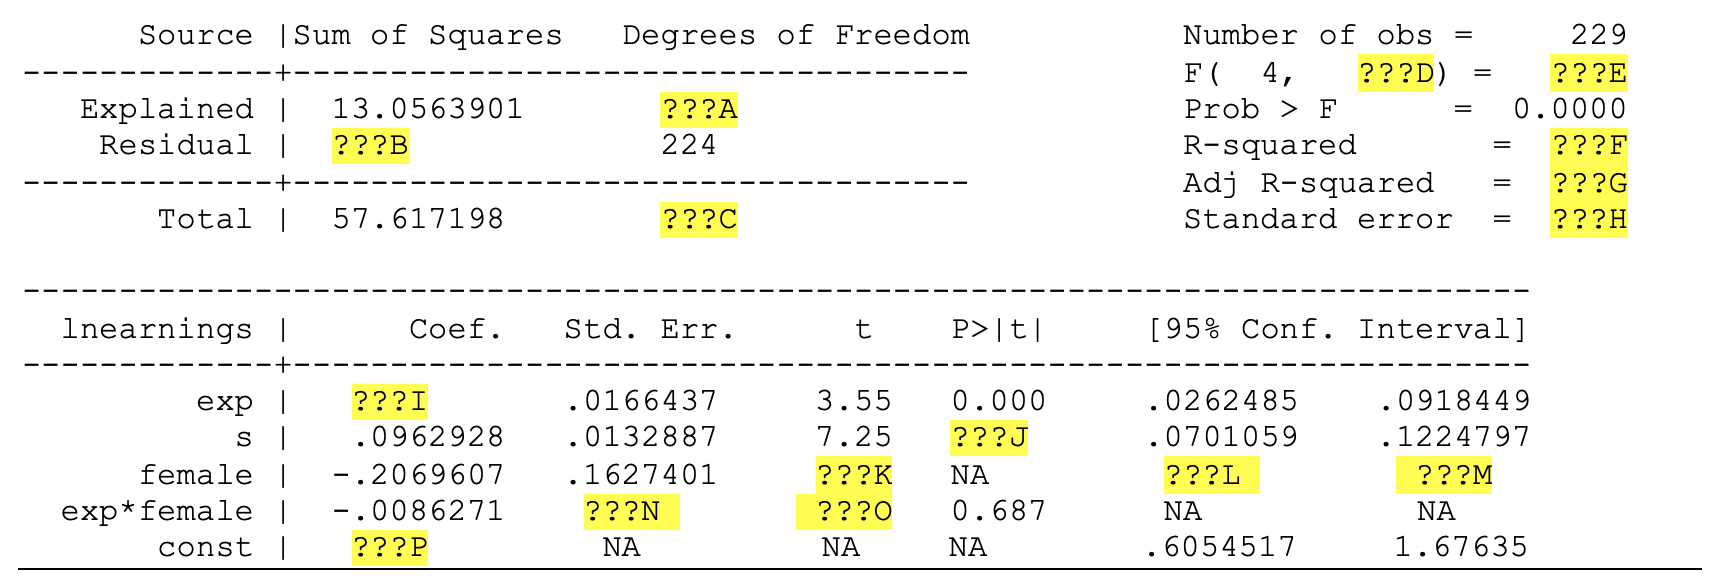
\includegraphics[scale=0.6]{figures/partial_stata_table.png}
    \end{minipage}

    That's the standard regression table reported by all software packages. 
    Here the letters $A$, $B$, \dots{ } just play the role of identifiers. 
    
    Reconstruct all the yellow entries with question marks. 
    

    \item Scared of proofs? That's Halloween, you should be scared!
    \begin{enumerate}
        \item Prove that in the simple regression $\hat y_i = \hb_0 + \hb_1 x_i$ the 
        standard $t$-statistic $t$ for the test $H_0$: $\beta_1 = 0$ and 
        the standard $F$-statistic $F$ for the same test satisfy the relation $t^2 = F$.
        \item Prove that in the simple regressions $\hat y_i = \hb_0 + \hb_1 x_i$ and 
        $\hat x_i = \hat{\gamma}_0 + \hat{\gamma}_1 y_i$ the determination coefficients are equal. 
    \end{enumerate}


    \item Consider the model $y = X\beta + u$ on the training set where $\beta$ is non-random,
    $\E(u \mid X) = 0$, the matrix $X$ of size $n\times k$ has $\rank X = k$, 
    but $\Var(u \mid X) = \sigma^2 I$, where $I$ is an identity matrix. 
    Observations are independent. 
    Let $\hb$ be the standard OLS estimator of $\beta$ using the training set data. 
    You have a test set with the same type of dependency $y' = X' \beta + u'$,
    $\E(u' \mid X') = 0$, $\Var(u' \mid X') = \sigma^2 I$.
    You make the forecast $\hat y'$ for the test set, $\hat y' = X' \hat\beta$.

    \begin{enumerate}
        \item Find $\E(\hat y' \mid X, X')$.
        \item Find $\Var(y' - \hat y' \mid X, X')$.
        \item Find $\Cov(\hb, y' - \hat y' \mid X, X')$.
    \end{enumerate}

    \item Let $u = (u_1, u_2, u_3)$ be the vector of iid standard normal random variables. 
    Denote the linear span of the vector $(1, 1, 0)$ be $V$.
    Let $W = V^{\perp}$ be the orthogonal complement of $V$ in $\RR^3$. 

    \begin{enumerate}
        \item Find $\dim V$, $\dim W$.
        \item Find the projection matrix $H$ that projects vectors from $\RR^3$ onto $V$.
    \end{enumerate}
    Let $v = Hu$ and $w = (I - H)u$.
    \begin{enumerate}[resume]
        \item Find the law of distribution of the random variables $v^T v$ and $\norm{w}^2$.
        \item Find the distribution of $2v^Tv/(w^Tw)$.
    \end{enumerate}

    \item Assume that the true model is $y_i = \beta_0 +  u_i$ and $u_i$ are iid normally distributed with zero mean and variance $\sigma^2$.
    There are $n$ observations.
    We estimate regression $\hat y_i = \hat \beta_0 + \hat\beta_1 x_i$ using OLS.

    \begin{enumerate}
        \item Find $\E(\hat \beta_1 \mid x)$  and $\E(\hat\beta_1)$.
        \item Find $\E(R^2)$.
        \item Find $\E(R^2_{adj})$ for the adjusted coefficient 
        \[
            R^2_{adj} = 1 - \frac{\SSR / (n - 2)}{\SST / (n - 1)}.
        \]
        
    \end{enumerate}

\end{enumerate}

\section*{Demo variant «Pumpkin» solution}
\begin{enumerate}
    \item 
    \begin{enumerate}
        \item The confidence interval for $\beta_x$ is $[0.2 - 1.96 \cdot \sqrt{4.5}, 0.2 + 1.96 \cdot \sqrt{4.5}]$.
        \item The confidence interval for conditional expected value of dependent variable is centered at conditional expected value:
        \[
        \hat\mu = \E(y \mid x = 1, b = -1, c = 2) = 3 + 0.2 \cdot 1 + 0.5 \cdot (-1) - 0.7 \cdot 2
        \]
        \[
        \hat v =
        \]
        Confidence interval is 
        \[
            [\hat\mu - 1.96 \sqrt{\hat v}, \hat\mu + 1.96 \sqrt{\hat v}].
        \]
        \item The test statistic is $t = \frac{\hb_x + \hb_b - 1}{\sqrt{\hVar(\hb_x) + \hVar(\hb_b) - 2 \hCov(\hb_x, \hb_b)}}$.
    \end{enumerate}

    \item 
    \begin{enumerate}
        \item $\E(\hb_1' \mid x) = \beta_1$
        \item $\hb_1'$ is consistent.
    \end{enumerate}

    \item 
    \begin{enumerate}
        \item $F = \frac{(500 - 300) / 3}{300 / (300 - 4)}$.
        \item $F = \frac{(300 - 250) / 2}{250 / (300 - 4)}$.
        \item $F = \frac{(300 - 150) / 100}{150 / (300 - 4 - 100)}$.
    \end{enumerate}

    \item 
    \begin{enumerate}
        \item % $\hb_0 = 1$, $\hb_1 = 2$.
        \item % $\SSR = 2$, $\SSE = 8$, $\SST = 10$, $R^2 = 1 - 0.2 = 0.8$.
        \item % $\hat \sigma^2 = 2/3$.
    \end{enumerate}
    \item
    \begin{enumerate}
        \item $\E(\hb \mid X) = \beta$, $\E(\hb) = \beta$.
        \item $\Var(\hb \mid X) = \sigma^2 (X'X)^{-1} X' W X (X'X)^{-1}$.
        \item No, it will not be valid as it is based on different covariance matrix of $\hb$.
        \item $\Cov(y, \hb \mid X) = ...$.
    \end{enumerate}
    \item 
    \begin{enumerate}
        \item Estimators $\hb_2$ and $\hat \gamma$ are equal.
        \item Residuals in both regressions are equal.
    \end{enumerate}
\end{enumerate}



\subsection{Demo variant «Pumpkin» solution}
\begin{enumerate}
\item 
\item 
\item 
\item 
\begin{enumerate}
    \item $\E(\hat y' \mid X, X') = X' \beta$.
    \item $\Var(y' - \hat y' \mid X, X') = ...$.
    \item $\Cov(\hb, y' - \hat y' \mid X, X') = -\Cov(\hb, X' \hb \mid X, X') = -(X^T X)^{-1}(X')^T$.
\end{enumerate}

\item 
\begin{enumerate}
    \item $\dim V = 1$, $\dim W = 2$.
    \item $H = \begin{pmatrix}
        1/2 & 1/2 & 0 \\
        1/2 & 1/2 & 0 \\
        0 & 0 & 0 \\
    \end{pmatrix}$.
    \item $v^Tv \sim \chi^2_1$, $\norm{w}^2 \sim \chi^2_2$.
    \item $2v^Tv/(w^Tw) \sim F_{1,2}$.
\end{enumerate}
\item 
\begin{enumerate}
    \item $\E(\hat\beta_1) = 0$, $\E(\hat\beta_1 \mid x) = 0$.
    \item $\E(R^2) = ...$. Should be positive :)
    \item $\E(R^2_{adj}) = 0$.
\end{enumerate}

\end{enumerate}


